\ylDisplay{Kärbes lendab} % Ülesande nimi
{EFO žürii} % Autor
{piirkonnavoor} % Voor
{2019} % Aasta
{P 9} % Ülesande nr.
{3} % Raskustase
{
% Teema: Valgusõpetus
\ifStatement
Kärbes asub kumerläätsest kümnekordse fookuskauguse kaugusel ning läätse optilisest peateljest kolme fookuskauguse kaugusel ning hakkab liikuma otse oma kujutise poole. Kui kaugel läätse tasandist asub kärbes hetkel, kui tema tõeline kujutis liigub kärbse suhtes \\
a) kõige aeglasemalt; \\
b) kõige kiiremini? Kui suur on kärbse kujutise kiirus nendel hetkedel?
\fi
\ifHint
Kuna kärbes lendab otse oma kujutise poole, siis peab ta lendama läätse keskpunkti poole. Kärbes ja tema kujutis asuvad alati sirgel.
\fi
\ifSolution
\begin{center}
	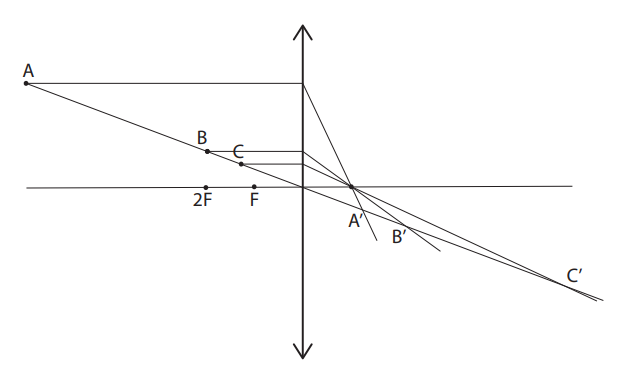
\includegraphics[width=0.5\linewidth]{2019-v2p-09-lah.PNG}
\end{center}
Kuna kärbes lendab otse oma kujutise poole, siis peab ta lendama läätse keskpunkti poole. Kärbes ja tema kujutis asuvad alati sirgel $AC'$. Kui kärbes lendab punktist $A$ punkti $B$, siis kujutis liigub punktist $A'$ punkti $B'$. Jooniselt on näha, et kärbse kujutis liigub aeglasemalt kui kärbes. Konstrueerides punktide $A$ ja $B$ vahele veel punkte on näha, et kujutise kiirus on järjest suureneb, kui kärbes läheneb punktile $B$. Kui kärbes asub läätsest kahekordse fookuskauguse kaugusel (punkt $B$), siis asub ka kujutis läätsest kahekordse fookuskauguse kaugusel (punkt $B'$). Sellises kohas on kärbse ja tema kujutise kiirused võrdsed, seega on kärbse ja tema kujutise kiirus teineteise suhtes $v_{min} = 0$ m/s. Kui kärbes liigub punktist $B$ fookaaltasandi suunas, siis kujutise kiirus järjest suureneb ning vahetult enne fokaaltasandile jõudmist on kujutise kiirus lõpmatult suur ($v_{max} = \infty$ m/s). Seega on kujutise kiirus kärbse suhtes maksimaalne siis, kui kärbes on väga lähedal fokaaltasandile ehk kärbes asub läätse tasandist fookuskauguse kaugusel.
\fi
}
